Java technology consists of the Java language definition, a
definition of the standard library, and the definition of an
intermediate instruction set with an accompanying execution
environment. This combination helps to make \emph{write once, run
anywhere} possible.

The following chapter gives a short overview of the Java programming
language. A more detailed description of the Java Virtual Machine
(JVM) and the explanation of the JVM instruction set, the so-called
bytecodes follows. The exploration of dynamic instruction counts of
typical Java programs can be found in Section~\ref{sec:bench:jvm}.

\section{Java}

Java is a relatively new and popular programming language. The main
features that have helped Java achieve success are listed below:
%
\begin{description}
    \item[Simple and object oriented:]
Java is a simple programming language that appears very similar to
C. This `look and feel' of C means that programmers that know C, can
switch to Java without difficulty. Java provides a simplified object
model with single inheritance\footnote{Java has \emph{single
inheritance} of \emph{implementation} -- only one class can be
extended. However, a class can implement several interfaces, which
means that Java has \emph{multiple interface inheritance}.}.

    \item[Portability:]
To accommodate the diversity of operating environments, the Java
compiler generates bytecodes -- an architecture neutral intermediate
format. To guarantee platform independence, Java specifies the sizes
of its basic data types and the behavior of its arithmetic
operators. A Java interpreter, the Java virtual machine, is
available on various platforms to help make `write once, run
anywhere' possible.

    \item[Availability:]
Java is not only available for different operating systems, it is
available at no cost. The runtime system and the compiler can be
downloaded from Sun's website for Windows, Linux and Solaris.
Sophisticated development environments, such as Netbeans or Eclipse,
are available under the GNU Public License.

    \item[Library:]
The complete Java system includes a rich class library to increase
programming productivity. Besides the functionality from a C
standard library, it also contains other tools, such as collection
classes and a GUI toolkit.

    \item[Built-in multithreading:]
Java supports multithreading at the language level: the library
provides the \code{Thread} class, the language provides the keyword
\code{synchronized} for critical sections and the runtime system
provides monitor and condition lock primitives. The system libraries
have been written to be thread-safe: the functionality provided by
the libraries is available without conflicts due to multiple
concurrent threads of execution.

    \item[Safety:]
Java provides extensive compile-time checking, followed by a second
level of runtime checking. The memory management model is simple --
objects are created with the \code{new} operator. There are no
explicit pointer data types and no pointer arithmetic, but there is
automatic garbage collection. This simple memory management model
eliminates a large number of the programming errors found in C and
C++ programs. A restricted runtime environment, the so-called
\emph{sandbox}, is available when executing small Java applications
in Web browsers.

\end{description}
%
\begin{figure*}
    \centering
    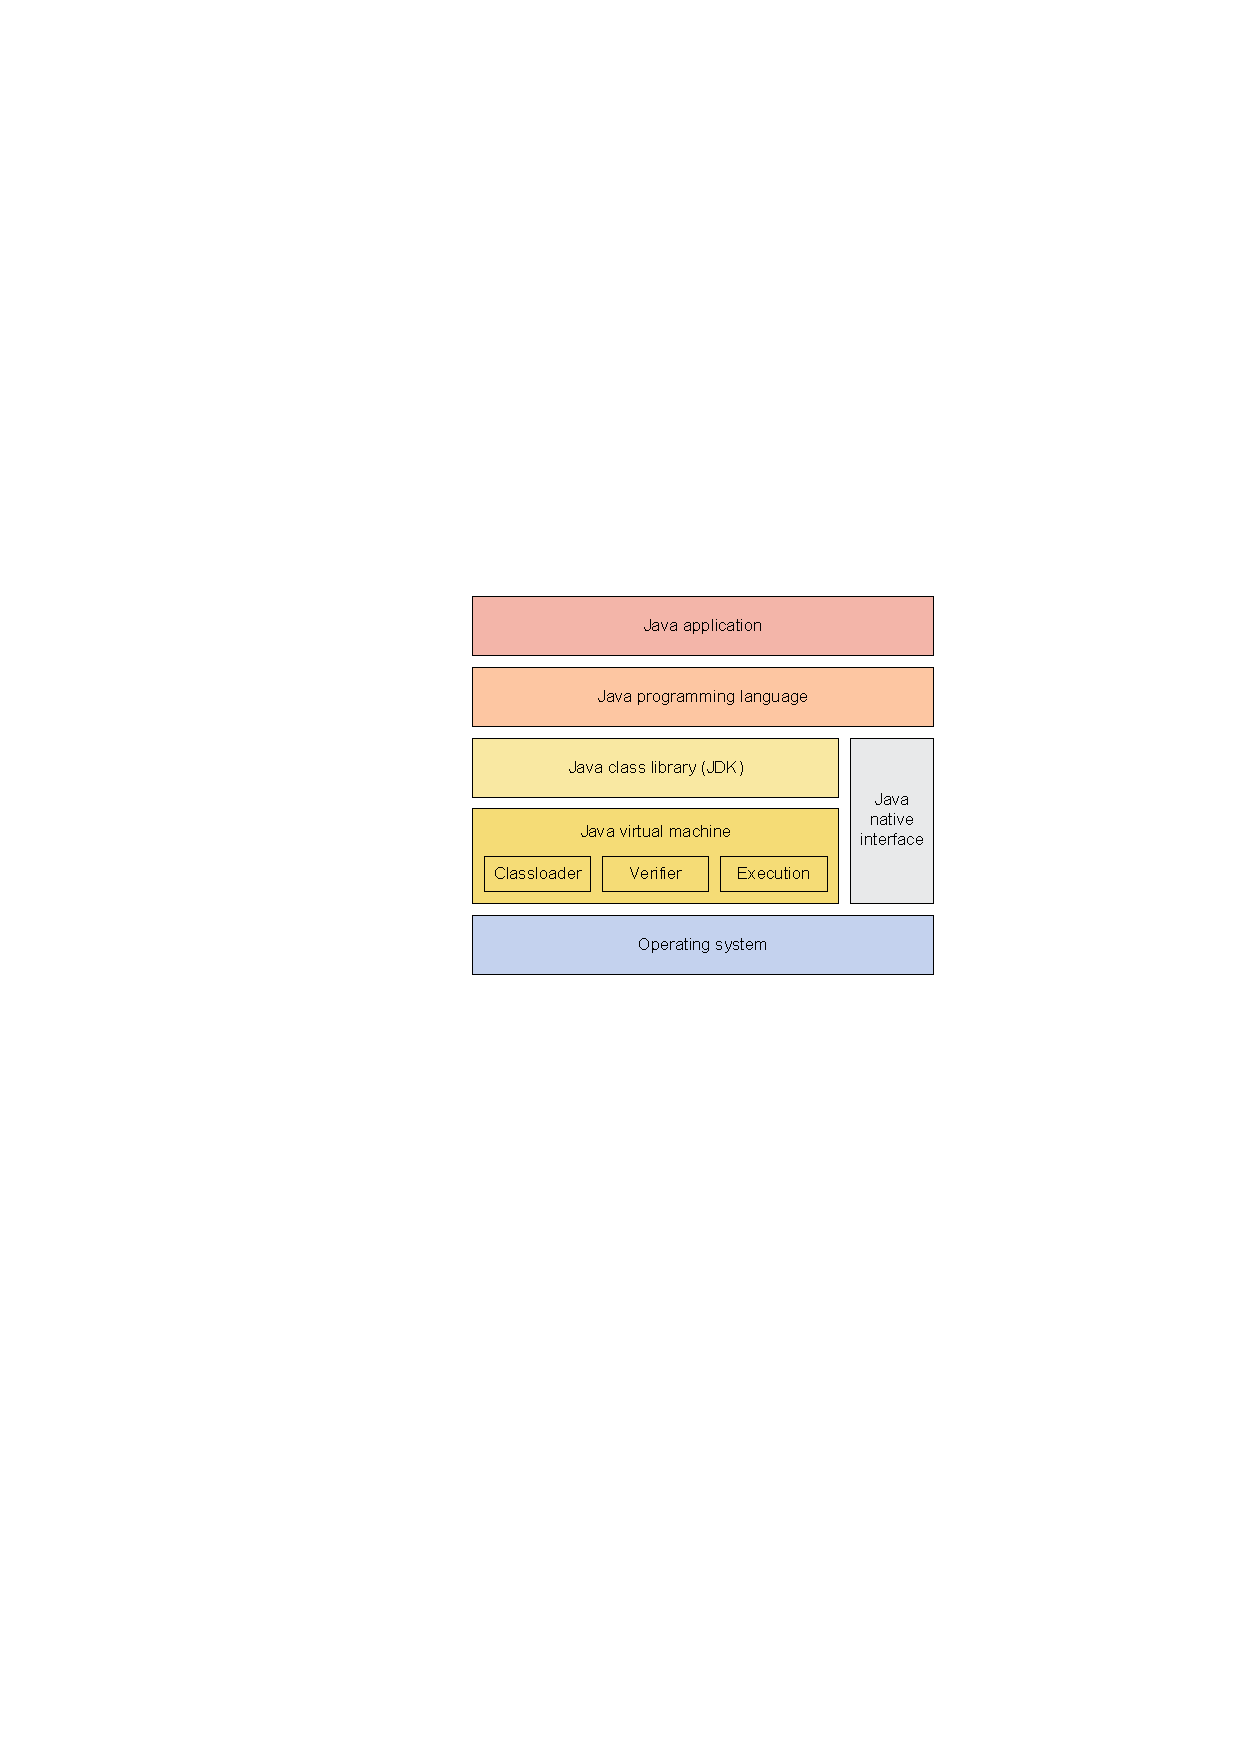
\includegraphics[scale=\picscale]{intro/java_overview}
    \caption{Java system overview}
    \label{fig:java:overview}
\end{figure*}
%
As can be seen in \figurename~\ref{fig:java:overview}, Java consists
of three main components:
%
\begin{enumerate}
    \item The Java programming language as defined in
    \cite{JavaLangSpec2}
    \item The class library, defined as part of the Java
    specification. All implementations of Java have to contain the
    library defined by Sun
    \item The Java virtual machine (defined in \cite{jvm}) that loads,
     verifies and executes the binary representation (the
\emph{class file}) of a Java program
\end{enumerate}
%
The Java native interface supports functions written in C or C++.
This combination is sometimes called \emph{Java technology} to
emphasize the fact that Java is more than just another
object-oriented language.

However, a number of issues have hindered a broad acceptance of
Java. The original presentation of Java as an Internet language led
to the misconception that Java was not a general-purpose programming
language. Another obstacle was the first implementation of the JVM
as an interpreter. Execution of Java programs was \emph{very} slow
compared to compiled C/C++ programs. Although advances in its
runtime technology, in particular the just-in-time compiler, have
closed the performance gap, it is still a commonly held view that
Java is slow.

\subsection{History}

The Java programming language originated as part of a research
project to develop software for network devices and embedded
systems. In the early '90s, Java, which was originally known as Oak
\cite{java:oak, java:oak2}, was created as a programming tool for a
consumer device that we would today call a PDA. The device (known as
*7) was a small SPARC-based hardware device with a tiny embedded OS.
However, the *7 was not issued as a product and Java was officially
released in 1995 as a new language for the Internet (to be
integrated into Netscape's browser). Over the years, Java technology
has become a programming tool for desktop applications, web servers
and server applications. These application domains resulted in the
split of the Java platform into the Java standard edition (J2SE) and
the enterprise edition (J2EE) in 1999. With every new release, the
library (defined as part of the language) continued to grow. Java
for embedded systems was clearly not an area Sun was interested in
pursuing. However, with the arrival of mobile phones, Sun again
became interested in this embedded market. Sun defined different
subsets of Java, which have now been combined into the Java Micro
Edition (J2ME). A detailed description of the J2ME follows in
Section~\ref{sec:j2me}.


\subsection{The Java Programming Language}

The Java programming language is a general-purpose object-oriented
language. Java is related to C and C++, but with a number of aspects
omitted. Java is a strongly typed language, which means that type
errors can be detected at compile time. Other errors, such as wrong
indices in an array, are checked at runtime. The
problematic\footnote{C pointers represent memory addresses as data.
Pointer arithmetic and direct access to memory leads to common and
hard-to-find program errors.} \emph{pointer} in C and explicit
deallocation of memory is completely avoided. The pointer is
replaced by a \emph{reference}, i.e.\ an abstract pointer to an
object. Storage for an object is allocated from the heap during
creation of the object with \code{new}. Memory is freed by automatic
storage management, typically using a garbage collector. The garbage
collector avoids memory leaks from a missing \code{free()} and the
safety problems exposed by dangling pointers.

The types in Java are divided into two categories: primitive types
and reference types. \tablename~\ref{tab:java:primitive} lists the
available primitive types. Method local variables, class fields and
object fields contain either a primitive type value or a reference
to an object.

\begin{table}
    \centering
    \begin{tabular}{ll}
        \toprule
        Type & Description \\
        \midrule
        \code{boolean} & either \code{true} or \code{false} \\
        \code{char} & 16-bit Unicode character (unsigned) \\
        \code{byte} & 8-bit integer (signed) \\
        \code{short} & 16-bit integer (signed) \\
        \code{int} & 32-bit integer (signed) \\
        \code{long} & 64-bit integer (signed) \\
        \code{float} & 32-bit floating-point (IEEE 754-1985) \\
        \code{double} & 64-bit floating-point (IEEE 754-1985) \\
        \bottomrule
    \end{tabular}
    \caption{Java primitive data types}
    \label{tab:java:primitive}
\end{table}

Classes and class instances, the objects, are the fundamental data
and code organization structures in Java. There are no global
variables or functions as there are in C/C++. Each method belongs to
a class. This `everything belongs to a class or an object' combined
with the class naming convention, as suggested by Sun, avoids name
conflicts in even the largest applications.

New classes can extend exactly one superclass. Classes that do not
explicitly extend a superclass become direct subclasses of
\code{Object}, the root of the whole class tree. This single
inheritance model is extended by \emph{interfaces}. Interfaces are
abstract classes that only define method signatures and provide no
implementation. A concrete class can implement several interfaces.
This model provides a simplified form of multiple inheritance.

Java supports multitasking through \emph{threads}. Each thread is a
separate flow of control, executing concurrently with all other
threads. A thread contains the method stack as thread local data --
all objects are shared between threads. Access conflicts to shared
data are avoided by the proper use of \code{synchronized} methods or
code blocks.

Java programs are compiled to a machine-independent bytecode
representation as defined in \cite{jvm}. Although this intermediate
representation is defined for Java, other programming languages
(e.g.\ ADA \cite{269646}) can also be compiled into Java bytecodes.

\section{The Java Virtual Machine}

The Java virtual machine (JVM) is a definition of an abstract
computing machine that executes bytecode programs. The JVM
specification \cite{jvm} defines three elements:
\begin{itemize}
    \item An instruction set and the meaning of those instructions
    -- the \emph{bytecodes}
    \item A binary format -- the \emph{class file} format. A
    class file contains the bytecodes, a symbol table and other
    ancillary information
    \item An algorithm to \emph{verify} that a class file
    contains valid programs
\end{itemize}
%
In the solution presented in this book, the class files are
verified, linked and transformed into an internal representation
before being executed on JOP. This transformation is performed with
\cmd{JOPizer} and is not executed on JOP. We will therefore omit the
description of the class file and the verification process.

The instruction set of the JVM is stack-based. All operations take
their arguments from the stack and put the result onto the stack.
Values are transferred between the stack and various memory areas.
We will discuss these memory areas first, followed by an explanation
of the instruction set.

\subsection{Memory Areas}

The JVM contains various runtime data areas. Some of these areas are
shared between threads, whereas other data areas exist separately
for each thread.

\begin{description}
    \item[Method area:]
The method area is shared among all threads. It contains static
class information such as field and method data, the code for the
methods and the constant pool. The constant pool is a per-class
table, containing various kinds of constants such as numeric values
or method and field references. The constant pool is similar to a
symbol table.

Part of this area, the code for the methods, is very frequently
accessed (during instruction fetch) and therefore is a good
candidate for caching.

    \item[Heap:]
The heap is the data area where all objects and arrays are
allocated. The heap is shared among all threads. A garbage collector
reclaims storage for objects.

    \item[JVM stack:]
Each thread has a private stack area that is created at the same
time as the thread. The JVM stack is a logical stack that contains
following elements:
\begin{enumerate}
    \item A frame that contains return information for a method
    \item A local variable area to hold local values inside a method
    \item The operand stack, where all operations are performed
\end{enumerate}
%
Although it is not strictly necessary to allocate all three elements
to the same type of memory we will see in Section~\ref{sec:stack}
that the argument-passing mechanism regulates the layout of the JVM
stack.

Local variables and the operand stack are accessed as frequently as
registers in a standard processor. A Java processor shall provide
some caching mechanism of this data area.

\end{description}
%
The memory areas are similar to the various segments in conventional
processes (e.g.\ the method code is analogous to the `text'
segment). However, the operand stack replaces the registers in a
conventional processor.

\subsection{JVM Instruction Set}

The instruction set of the JVM contains 201 different instructions
\cite{jvm}, the \emph{bytecodes} that can be grouped into the
following categories:
%
\begin{description}
    \item[Load and store:]
Load instructions push values from the local variables onto the
operand stack. Store instructions transfer values from the stack
back to local variables. 70 different instructions belong to this
category. Short versions (single byte) exist to access the first
four local variables. There are unique instructions for each basic
type (\code{int}, \code{long}, \code{float}, \code{double} and
\code{reference}). This differentiation is necessary for the
bytecode verifier, but is not needed during execution. For example
\code{iload}, \code{fload} and \code{aload} all transfer one 32-bit
word from a local variable to the operand stack.

    \item[Arithmetic:]
The arithmetic instructions operate on the values found on the stack
and push the result back onto the operand stack. There are
arithmetic instructions for \code{int}, \code{float} and
\code{double}. There is no direct support for \code{byte},
\code{short} or \code{char} types. These values are handled by
\code{int} operations and have to be converted back before being
stored in a local variable or an object field.

    \item[Type conversion:]
The type conversion instructions perform numerical conversions
between all Java types: as implicit widening conversions (e.g.\
\code{int} to \code{long}, \code{float} or \code{double}) or
explicit (by casting to a type) narrowing conversions.

    \item[Object creation and manipulation:]
Class instances and arrays (that are also objects) are created and
manipulated with different instructions. Objects and class fields
are accessed with type-less instructions.

    \item[Operand stack manipulation:]
All direct stack manipulation instructions are type-less and
operate on 32-bit or 64-bit entities on the stack. Examples of these
instructions are \code{dup}, to duplicate the top operand stack
value, and \code{pop}, to remove the top operand stack value.

    \item[Control transfer:]
Conditional and unconditional branches cause the JVM to continue
execution with an instruction other than the one immediately
following. Branch target addresses are specified relative to the
current address with a signed 16-bit offset. The JVM provides a
complete set of branch conditions for \code{int} values and
references. Floating-point values and type \code{long} are
supported through compare instructions. These compare instructions
result in an \code{int} value on the operand stack.

    \item[Method invocation and return:]
The different types of methods are supported by four instructions:
invoke a class method, invoke an instance method, invoke a method
that implements an interface and an \code{invokespecial} for an
instance method that requires special handling, such as
\code{private} methods or a superclass method.


\end{description}
%
A bytecode consists of one instruction byte followed by optional
operand bytes. The length of the operand is one or two bytes, with
the following exceptions: \code{multianewarray} contains 3 operand
bytes; \code{invokeinterface} contains 4 operand bytes, where one is
redundant and one is always zero; \code{lookupswitch} and
\code{tableswitch} (used to implement the Java \code{switch}
statement) are variable-length instructions; and \code{goto\_w} and
\code{jsr\_w} are followed by a 4 byte branch offset, but neither is
used in practice as other factors limit the method size to 65535
bytes.

\subsection{Methods}

A Java \emph{method} is equivalent to a \emph{function} or
\emph{procedure} in other languages. In object oriented terminology
this \emph{method} is \emph{invoked} instead of \emph{called}. We
will use \emph{method} and \emph{invoke} in the remainder of this
text. In Java and the JVM, there are five types of methods:
%
\begin{itemize}
    \item Static or class methods
    \item Virtual methods
    \item Interface methods
    \item Class initialization
    \item Constructor of the parent class (\code{super()})
\end{itemize}
%
For these five types there are only four different bytecodes:
\begin{description}
    \item[\code{invokestatic}:] A class method (declared \code{static})
    is invoked. As the target does not depend on an object, the
    method reference can be resolved at load/link time.

    \item[\code{invokevirtual}:] An object reference is resolved and
    the corresponding method is invoked. The resolution is usually
    done with a dispatch table per class containing all implemented and
    inherited methods. With this dispatch table, the resolution can
    be performed in constant time.

    \item[\code{invokeinterface}:] An interface allows Java
    to emulate multiple inheritance. A class can implement several
    interfaces, and different classes (that have no inheritance
    relation) can implement the same interface. This flexibility
    results in a more complex resolution process. One method of
    resolution is a search through the class hierarchy that results
    in a variable, and possibly lengthy, execution time. A constant time
    resolution is possible by assigning every interface method a
    unique number. Each class that implements an interface needs its
    own table with unique positions for each interface method of
    the \emph{whole} application.

    \item[\code{invokespecial}:] Invokes an instance method with
    special handling for superclass, \code{private}, and instance
    initialization. This bytecode catches many different cases.
    This results in expensive checks for common \code{private} instance
    methods.
\end{description}
%

\subsection{Implementation of the JVM}

There are several different ways to implement a virtual machine. The
following list presents these possibilities and analyses how
appropriate they are for embedded devices.
%
\begin{description}
    \item[Interpreter:]
The simplest realization of the JVM is a program that interprets the
bytecode instructions. The interpreter itself is usually written in
C and is therefore easy to port to a new computer system. The
interpreter is very compact, making this solution a primary choice
for resource-constrained systems. The main disadvantage is the high
execution overhead. From a code fragment of the typical interpreter
loop, as shown in Listing~\ref{lst:intro:java:intprt}, we can
examine the overhead: The emulation of the stack in a high-level
language results in three memory accesses for a simple \code{iadd}
bytecode. The instruction is decoded through an indirect jump.
Indirect jumps are still a burden for standard branch prediction
logic.

\begin{lstlisting}[float,caption={Typical JVM interpreter loop},
label=lst:intro:java:intprt]
    for (;;) {
        instr = bcode[pc++];
        switch (instr) {
            ...
            case IADD:
                tos = stack[sp]+stack[sp-1];
                --sp;
                stack[sp] = tos;
                break;
            ...
        }
    }
\end{lstlisting}

    \item[Just-In-Time Compilation:]
Interpreting JVMs can be enhanced with just-in-time (JIT) compilers.
A JIT compiler translates Java bytecodes to native instructions
during runtime. The time spent on compilation is part of the
application execution time. JIT compilers are therefore restricted
in their optimization capacity. To reduce the compilation overhead,
current JVMs operate in mixed mode: Java methods are executed in
interpreter mode and the call frequency is monitored. Often-called
methods, the hot spots, are then compiled to native code.

JIT compilation has several disadvantages for embedded systems,
notably that a compiler (with the intrinsic memory overhead) is
necessary on the target system. Due to compilation during runtime,
execution times are not predictable\footnote{Even if the time for
the compilation is known, the WCET for a method has to include the
compile time!}.

    \item[Batch Compilation:]
Java can be compiled, in advance, to the native instruction set of
the target. Precompiled libraries are linked with the application
during runtime. This is quite similar to C/C++ applications with
shared libraries. This solution undermines the flexibility of Java:
dynamic class loading during runtime. However, this is not a major
concern for embedded systems.


    \item[Hardware Implementation:]
A Java processor is the implementation of the JVM in hardware. The
JVM bytecode is the native instruction set of such a processor. This
solution can result in quite a small processor, as a stack
architecture can be implemented very efficiently. A Java processor
is memory-efficient as an interpreting JVM, but avoids the execution
overhead. The main disadvantage of a Java processor is the lack of
capability to execute C/C++ programs.

\end{description}

\subsection{Embedded Java}

\begin{figure}
    \centering
    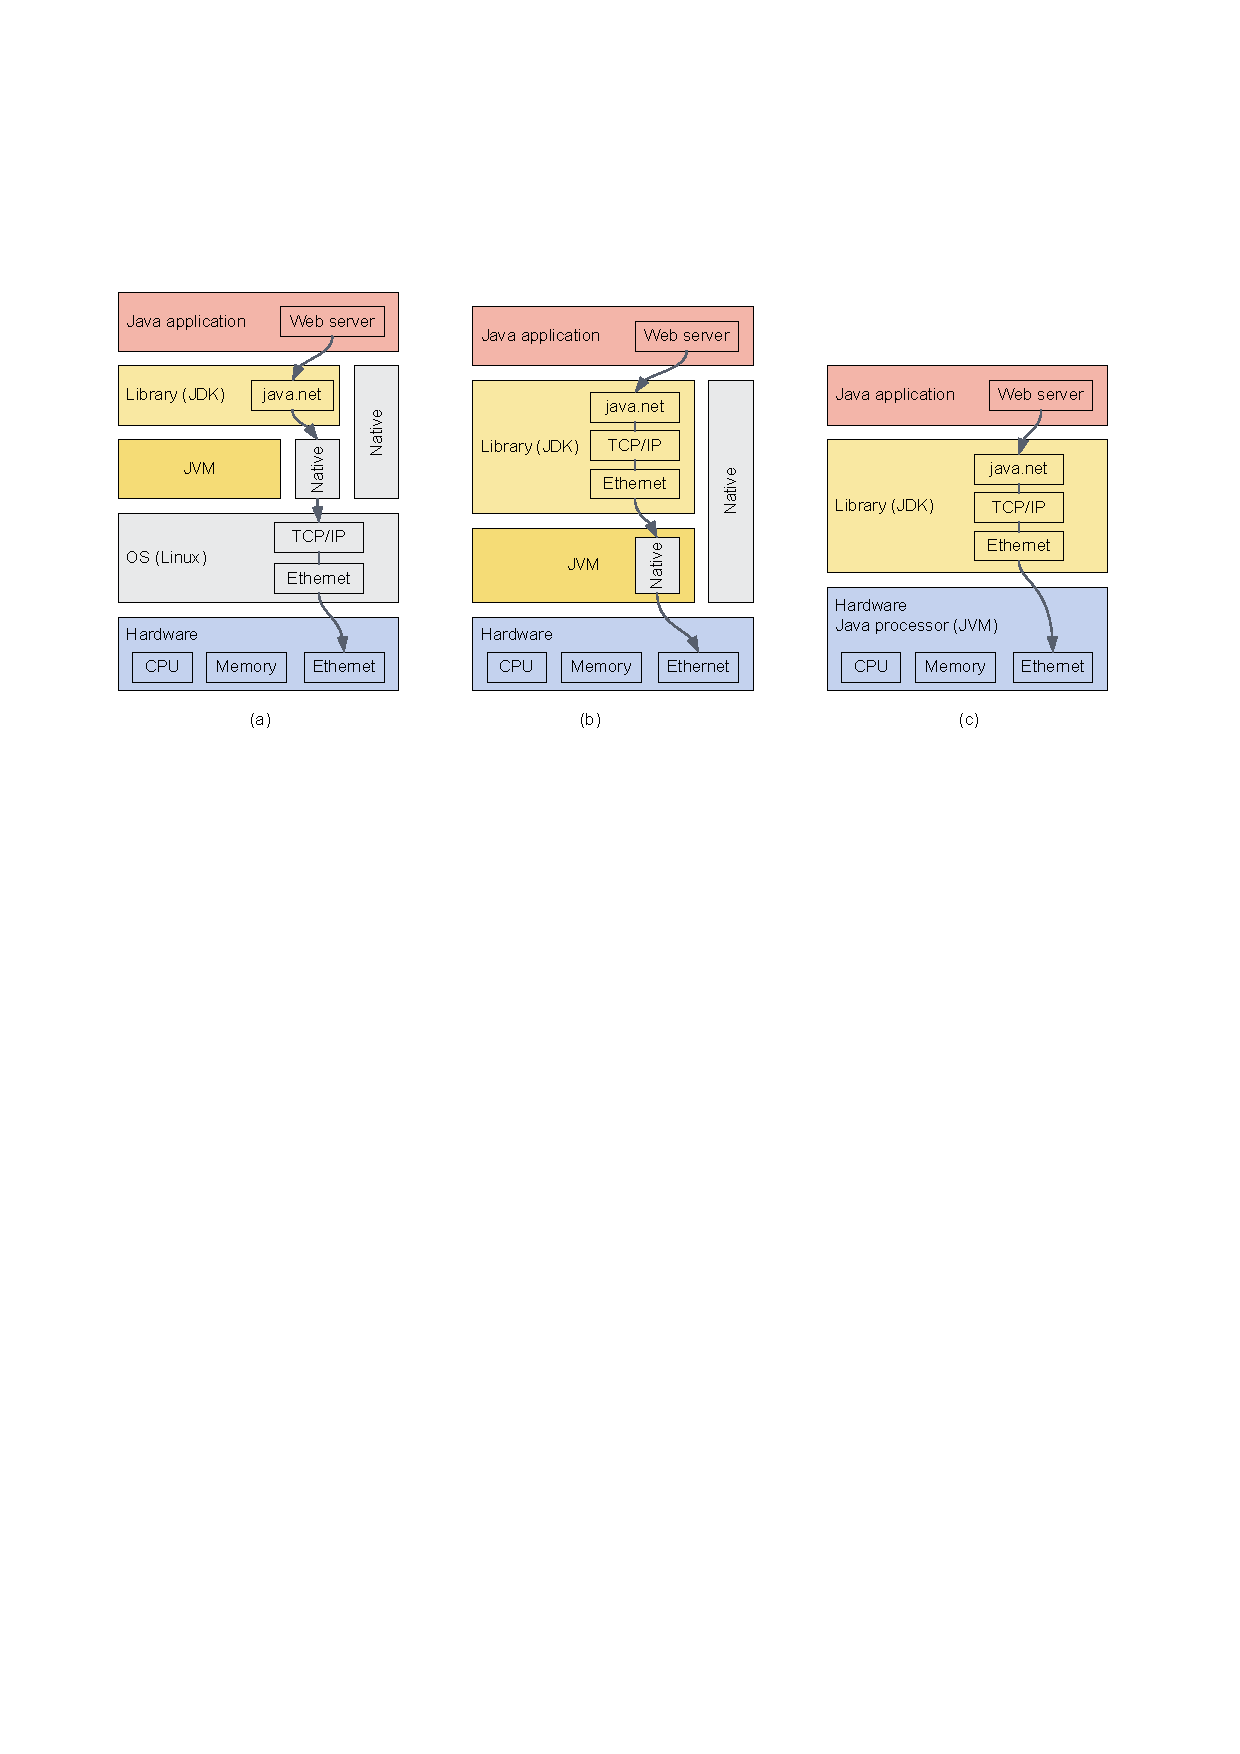
\includegraphics[width=\textwidth]{visio/jvmall}
    \caption{Implementation variations of Java in embedded systems}\label{fig:java:embedded}
\end{figure}

In embedded systems the architecture of JVMs are more diverse than
on desktop or server systems. Figure~\ref{fig:java:embedded} shows
variations of Java implementations in embedded systems and an
example of the control flow for a web server application. The
standard approach of a JVM running on top of an operating system
(OS) is shown in sub-figure (a). A network connection bypasses the
JVM via native functions and uses the TCP/IP stack implementation
and the device drivers of the OS.

A JVM without and OS is shown in sub-figure (b). This solution is
often called \emph{running on the bare metal}. The JVM acts as the
OS and provides the thread scheduling and the low-level access to
the hardware. In that case the network stack can be written entirely
in Java. JNode\footnote{\url{http://www.jnode.org/}} is an approach
to implement the OS entirely in Java. This solution becomes popular
even in server
applications\footnote{\url{http://www.bea.com/framework.jsp?CNT=index.htm&FP=/content/products/weblogic/virtual_server}
}.

Sub-figure (c) shows an embedded solution where the JVM is part of
the hardware layer. That means it is implemented in a Java
processor. With this solution the native layer can be completely
avoided and all code (application and system code) is written
entirely in Java.

Figure~\ref{fig:java:embedded} shows how the flow from the
application goes down to the hardware. The example consists of a web
server and an Internet connection via Ethernet. In case (a) the
application web server talks with \code{java.net} in the JDK. The
flow goes down via a native interface to the TCP/IP implementation
and the Ethernet device driver within the OS (usually written in C).
The device driver talks with the Ethernet chip. In (b) the OS layer
is omitted: the TCP/IP layer and the Ethernet device driver are now
part of the Java library. In (c) the JVM is part of the hardware
layer and a direct access from the Ethernet driver to the Ethernet
hardware is mandatory. Note how part of the network stack moves up
from the OS layer to the Java library. Version (c) shows a pure Java
implementation of the whole network stack.


\section{Summary}

Java is a unique combination of the language definition, a rich
class library and a runtime environment. A Java program is compiled
to bytecodes that are executed by a Java virtual machine. Strong
typing, runtime checks and avoidance of pointers make Java a
\emph{safe} language. The intermediate bytecode representation
simplifies porting of Java to different computer systems. An
interpreting JVM is easy to implement and needs few system
resources. However, the execution speed suffers from interpreting.
JVMs with a just-in-time compiler are state-of-the-art for desktop
and server systems. These compilers require large amounts of memory
and have to be ported for each processor architecture, which means
they are not the best choice for embedded systems. A Java processor
is the implementation of the JVM as a concrete machine. A Java
processor avoids the slow execution model of an interpreting JVM and
the memory requirements of a compiler, thus making it an interesting
execution system for Java in embedded systems.
